\vspace{-4mm}
\section{APART Framework}
\vspace{-1mm}
\label{sec:framework}

<<<<<<< HEAD
In a real-time ride-sharing application, once the server receives a request, it needs to determine the driver who can best accommodate the new request with respect to his current schedule. With a large number of candidate drivers, the scheduling phase becomes the bottleneck in centralized frameworks where one single server processes the requests. Therefore, we introduce APART which overcomes this shortcoming by distributing the scheduling task to the drivers themselves. We first explain the auction framework in which the server broadcasts new arriving requests to the drivers. Subsequently, we discuss how each driver generates a bid based on its current schedule.
=======
In a real-time ride-sharing application, once the server receives a request, it needs to determine the driver who can best accommodate the new request with respect to his current schedule. With a large number of candidate drivers, the scheduling phase becomes the bottleneck in centralized frameworks where there is a single server processing the requests. Therefore, we introduce APART which overcomes this shortcoming by distributing the scheduling task to the drivers themselves. We first explain the auction framework in which the server broadcasts new arriving requests to the drivers. Subsequently, we discuss how each driver generates a bid based on its current schedule.
>>>>>>> 46f67d188a36b6f09f72c25697c415296ddf3444

\subsection{Dispatch Requests}
\label{subsec:dispatch}
Auction frameworks have been effectively used for assignment problems \cite{Lagoudakis04,Mehta05}. Following the terminology used in auction frameworks, APART considers drivers as bidders and ride requests as goods. Note that the actual human driver does not engage in bidding, instead, his mobile app software does the bidding based on various constraints and goals. The server plays the role of a central auctioneer in APART. With APART, once a new request is received by the server (auctioneer), it presents the request to the drivers (bidders). Each driver computes a new schedule which incorporates the incoming request, and generates a bid based on the driver's and riders' profile. Subsequently the bid is submitted to the server. The bidding process is performed as a \textit{sealed-bid auction} where drivers simultaneously submit bids and no other driver knows how much the other drivers have bid. In the end the server selects the driver with the highest bid as the winner and matches the request with the driver.

<<<<<<< HEAD
=======
Auction frameworks have been effectively used for assignment problems \cite{Lagoudakis04,Mehta05}. Following the terminology used in auction frameworks, APART considers drivers as bidders and ride requests as goods. Note that the actual human driver does not engage in bidding, instead, his mobile app software does the bidding based on various constraints and goals. The server plays the role of a central auctioneer in APART. With APART, once a new request is received by the server (auctioneer), it presents the request to the drivers (bidders). Each driver computes a new schedule which incorporates the incoming request, and generates a bid based on the driver's and riders' profile. Subsequently the bid is submitted to the server. The bidding process is performed as a \textit{sealed-bid auction} where drivers simultaneously submit bids and no other driver knows how much the other drivers have bid. In the end the server selects the driver with the highest bid as the winner and matches the request with the driver.

>>>>>>> 46f67d188a36b6f09f72c25697c415296ddf3444
With APART, drivers that are far away from the pick-up location of an incoming request, are not asked to bid on the request. The server only sends an incoming request to \textit{eligible drivers} that are defined as:
%With APART, the server does not need to know the exact location of every driver as it is not responsible for performing the scheduling phase. Consequently, APART utilized a grid index which only keeps track of which grid cell a driver is located in. Therefore, compared to a centralized setting where the exact location of every driver is stored, APART's grid index requires fewer updates and less maintenance, which further reduces the load on the server.

\begin{definition} [Eligible Drivers]
An available driver $v$ is said to be eligible for servicing a newly submitted request $r$, if and only if:
\vspace{-2mm}
\begin{equation*}
distance(v, r.s) \leq r.w \times avg\_speed
\end{equation*}
\end{definition}

<<<<<<< HEAD
\vspace{-2mm}
=======
\noindent In other words, an available driver \textit{d} is eligible for serving request \textit{r}, if he has enough time to reach the pick-up location of \textit{r} within \textit{r}'s waiting time. In order to find eligible workers for each request, the server maintains a spatial index on the location of the drivers. With APART, the server does not need to know the exact location of the drivers to be able to filter out non-eligible drivers. We use a grid index where the server only keeps track of which cell a driver is located in. For example, in \cref{fig:grid_index}, assuming the black dot is the pick-up location of a new request and $r$ is the maximum wait time for the new request, any driver in the shaded cells will receive the new request. In our grid index, we use the filter and refine process in \cite{Demiryurek09} in order to enable continuous query processing on the underlying road network using Euclidean distances.

>>>>>>> 46f67d188a36b6f09f72c25697c415296ddf3444
\begin{figure}[!ht]
	\centering
	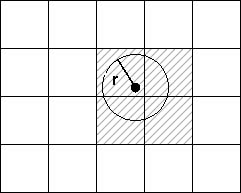
\includegraphics[width=0.35\columnwidth]{fig/grid_index.jpg}
	\vspace{-0mm}\caption{Spatiotemporal Grid Index} \vspace{-2mm} \label{fig:grid_index}
\end{figure}\vspace{-0mm}

\noindent In other words, an available driver \textit{d} is eligible for serving request \textit{r}, if he has enough time to reach the pick-up location of \textit{r} within \textit{r}'s waiting time. In order to find eligible workers for each request, the server maintains a spatial index on the location of the drivers. With APART, the server does not need to know the exact location of the drivers to filter out non-eligible drivers. We use a grid index where the server only keeps track of which cell a driver is located in. For example, in \cref{fig:grid_index}, assuming the black dot is the pick-up location of a new request and $r$ is the maximum wait time for the new request, any driver in the shaded cells will receive the new request. In our grid index, we use the filter and refine process in \cite{Demiryurek09} in order to enable continuous query processing on the underlying road network using Euclidean distances.

\begin{algorithm}
<<<<<<< HEAD
\caption{Dispatch($V_r, r, startTime$)}
\label{algo:dispatch}
\begin{algorithmic}[1]
\REQUIRE $V_r$ is the set of currently available drivers, $r$ is a new request and $startTime$ is the current time
\ENSURE $v \in V_r$ as the driver that request $r$ is assigned to
\STATE $v_{selected} \leftarrow $ \emph{null}
\STATE $Bids \leftarrow \emptyset$
\FOR{$v \in V_r$} \label{line:loop_start}
	\STATE $b_v \leftarrow $ ComputeBid$(v, v.schedule, r, startTime)$ \label{line:compute}
	\STATE $Bids \leftarrow Bids \cup \{b_v\}$
=======
\caption{Dispatch($V, r, time$)}
\label{algo:dispatch}
\begin{algorithmic}[1]
\REQUIRE $V$ is the set of currently available drivers, $r$ is a new request and $time$ is the current time
\ENSURE $v \in V$ as the driver which request $r$ should be assigned to
\STATE $v_{selected} = $ \emph{null}
\STATE $Bids = \emptyset$
\FOR{$v \in V_r$} \label{line:loop_start}
	\STATE $b_v = $ComputeBid$(v, r, time)$ \label{line:compute}
	\STATE $Bids \leftarrow  b_v$
>>>>>>> 46f67d188a36b6f09f72c25697c415296ddf3444
\ENDFOR \label{line:loop_end}
\STATE $v_{selected} \leftarrow \argmax_x \left\lbrace b_x \in Bids \right\rbrace$ \label{line:select}
\RETURN $v_{selected}$
\end{algorithmic}
\end{algorithm}
<<<<<<< HEAD
\vspace{-3mm}
\cref{algo:dispatch} outlines the process of assigning an incoming request $r$, where $V_r$ is the set of eligible drivers for request $r$ (line~\ref{line:loop_start}). For each candidate driver $v$, the \emph{ComputeBid} method (line \ref{line:compute}) is executed to perform scheduling and compute $v$'s bid (\cref{subsec:bidcomp}). Subsequently, the platform chooses the driver with the highest bid. In case of a tie in line \ref{line:select}, the algorithm randomly selects one driver among the ones with the highest bid. Notice that all the iterations of the \textbf{for} loop in \cref{algo:dispatch} (lines \ref{line:loop_start}-\ref{line:loop_end}) run in parallel.
=======

\cref{algo:dispatch} outlines the process of assigning an incoming request $r$. $V_r$ is the set of eligible drivers for request $r$ (line~\ref{line:loop_start}). Notice that all the iterations of the \textbf{for} loop in \cref{algo:dispatch} (lines \ref{line:loop_start}-\ref{line:loop_end}) run in parallel. The \emph{ComputeBid()} method (line \ref{line:compute}) that each driver executes, performs scheduling and computes the highest profit $v$ can generate for the platform (\cref{subsec:bidcomp}). In case of a tie in line \ref{line:select}, the algorithm randomly selects one driver among the ones with the highest bid.
>>>>>>> 46f67d188a36b6f09f72c25697c415296ddf3444

\subsection{Bid Computation \& Payments}
\label{subsec:bidcomp}

<<<<<<< HEAD
Once a driver is notified of a new request, it has to compute a bid. The bid each driver generates reflects the profit the system can gain if the request is assigned to that driver. Once the ride-sharing application receives the request, it generates a bid and submits the bid to the server. When a new request is assigned to a diver, he will be notified with an updated schedule. This means that the human driver's interaction with APART is limited to configuring his profile on the ride-sharing application.

%\begin{algorithm}[!h]
%\caption{ComputeBid($v, r, time$)}
%\label{algo:comp_bid}
%\begin{algorithmic}[1]
%\REQUIRE $v$ is a driver, $r$ is a new request and $time$ is the current time.
%\ENSURE additional $profit$ that $v$ can generate by accepting $r$
%\STATE $src = \lbrace r'.s | r' \in v.schedule \rbrace$ 
%\STATE $src.$add$(r.s)$
%\STATE \small{$profit_n, schedule = $FindBestSchedule$(\emptyset, src, -\infty, \emptyset,  time)$} \label{ln:fbs}
%\STATE $profit_c, cost_c = $GetProfitAndCost$(v.schedule, time)$ \label{ln:gps}
%\RETURN $profit_n - profit_c$
%\end{algorithmic}
%\end{algorithm}
%
%\vspace{-.2in}
%
%\begin{algorithm}[!h]
%\caption{GetProfitAndCost($schedule, start$)}
%\label{algo:get_profit}
%\begin{algorithmic}[1]
%\REQUIRE \emph{schedule} is an ordered list of pick-up/drop-off points and \emph{start} is the current time.
%\ENSURE a pair of ($profit, cost$) of performing the input schedule. If the input schedule is not valid it returns ($-\infty, \infty$)
%\STATE $time = start$
%\STATE $loc = v.$loc\label{ln:loc}
%\STATE $trip = 0$
%\FOR{$p$ \textbf{in} $schedule$}
%	\STATE $path =$ ShortestPath($loc, p$.loc)
%	\STATE $trip \pluseq$ Distance($path$)
%	\STATE $time \pluseq$ TravelTime($path$)
%	\IF{$p$.type $= start$}
%		\IF{$time > p$.req.req\_time $+ p$.req.w}
%			\RETURN $-\infty$
%		\ENDIF
%		\STATE $pickUp[p$.req$]=trip$
%	\ENDIF
%	\IF{$p$.type $= end$}
%		\STATE $\delta d = trip - pickUp[p$.req$]$
%		\STATE $fare \pluseq p$.f($\delta d$) $\times$ F($p$.req.sp)
%		\STATE $cost = v$.g($trip$)\label{ln:dprof}
%	\ENDIF
%\ENDFOR
%\STATE $profit = fare - cost$
%\RETURN $profit, cost$
%\end{algorithmic}
%\end{algorithm}
%
%\cref{algo:comp_bid} outlines the bid computation process. The \textit{FindBestSchedule()} method takes a list of pick-up locations of requests and finds the best valid schedule for those requests (line~\ref{ln:fbs}). The reason \textit{FindBestSchedule()} is initially called with only the pick-up locations is to guarantee, for every request its pick-up locations is scheduled before its drop-off locations. In \cref{algo:can_schedule}, once the pick-up location of a request is scheduled, its drop-off location is added to list of remaining nodes to be scheduled. The variable $profit_n$ is the total profit of the best valid schedule that contains $r$. However the profit of $v$'s current schedule should be deducted from $profit_n$ to give the additional profit $v$ can generate by accepting $r$. The \textit{GetProfitAndCost()} method computes the profit and cost of \textit{v}'s current schedule (line~\ref{ln:gps}).
%
%%At each point in time, every driver has a schedule $s$. For every request $r_j \in s$, the driver can determine $r_j$'s incurred detour in $s$. Subsequently, using \cref{eq:fare,eq:payment,eq:profit} the driver can compute the profit it makes for APART.
%
%\cref{algo:get_profit} outlines the process of determining the profit each driver can generate if he starts executing the input \textit{schedule} at time \textit{start}. Each driver $v$ runs this algorithm locally and hence, $v.loc$ (line~\ref{ln:loc}) and $v.g()$ (line~\ref{ln:dprof}) refer to $v$'s current location and profile, respectively. Also, whether $p$ is a pick-up or drop-off point, in \cref{algo:get_profit} $p.req$ refers to the request for which $p$ is one of the end points. \cref{algo:get_profit} goes through the nodes in \textit{schedule} one by one and for every drop-off node, computes the traveled distance from when the pick-up node was passed and using \cref{eq:fare,eq:payment,eq:profit}, \cref{algo:get_profit} can compute the profit and cost of \textit{schedule}. If the input \textit{schedule} is not valid, the algorithm returns $-\infty$ and $\infty$ as the profit and cost, respectively.
%
%\begin{algorithm}[!ht]
%\caption{FindBestSchedule($f, r, bp, bs, start$)}
%\label{algo:can_schedule}
%\begin{algorithmic}[1]
%\REQUIRE \emph{f} and \emph{r} are lists of pick-up/drop-off points that have been added and to be added to a valid schedule, respectively. \emph{bp} and \emph{bs} are the best profit and corresponding schedule observed so far and \emph{start} is the current time.
%\ENSURE $bp, bs$ as the best profit and corresponding schedule for input points is a valid schedule exists. Otherwise $-\infty, \emptyset$
%\IF{$f$.size $+ r$.size $ > v$.n $\times 2$}
%	\RETURN $bp, bs$
%\ENDIF
%\FOR{$p$ \textbf{in} $r$}
%	\STATE $f' = f$
%	\STATE $f'$.add($p$)
%	\STATE $p, c =$ GetProfitAndCost($f', start$)
%	\IF{$p \neq -\infty$ and $p \geq bp$}
%		\STATE $r' = r$
%		\STATE $r'$.remove($p$)
%		\IF{$p$.type $= start$}
%			\STATE $r'$.add($p$.req.end)\label{ln:dropoff}
%		\ENDIF
%		\IF{$r'$.size $= 0$}
%			\RETURN $p, f'$
%		\ENDIF
%		\STATE $p, s =$ FindBestSchedule($f', r', bp, bs, start$)
%		\IF{$p > bp$}
%			\STATE $bs = s$
%			\STATE $bp = p$
%		\ENDIF
%	\ENDIF
%\ENDFOR
%\RETURN $bp, bs$
%\end{algorithmic}
%\end{algorithm}
%
%The first step in computing a bid is to find a potential valid schedule. If multiple such schedules exist, the one which generates maximum profit should be selected. In order to find a valid schedule, each driver runs a branch and bound algorithm outlined in \cref{algo:can_schedule}. The algorithm recursively performs an exhaustive search to find the best valid schedule. The variable $f$ is the set of nodes that have already been added to the schedule and $r$ is the set of remaining nodes. In each call, one node from $r$ is added to $f$. Every time a new node is added to $f$, the algorithm checks if $f$, which is a partial schedule, is valid or not. If not valid, it does not proceed further on that branch and backtracks to one level higher. The algorithm starts by only pick-up nodes of the requests in $r$ to ensure the pick-up node of a request is scheduled before its drop-off node. Once the pick-up node of a request is added to $f$, the drop-off node of the same request is added to $r$ (Line~\ref{ln:dropoff}).
%
%Once drivers submit their bids, the server selects the driver with the highest bid as the winner and assigns the new request to that. Assuming driver $v$ wins the auction, his reward for serving the request is the same amount as $cost_v$, based on which he determined the bid value. Also, upon assigning the new request to $v$, the service providers increases its revenue by $b_v$.


%%%%%%
%%% Ding's vesion of computing bid.
\begin{algorithm}[!h]
	\caption{ComputeBid($v, v.schedule, r, startTime$)}
	\label{algo:comp_bid}
	\begin{algorithmic}[1]
		\REQUIRE $v$ is a driver with schedule $v.schedule$, $r$ is a new request and $start\_time$ is the current time.
		\ENSURE additional $profit$ that $v$ can generate by accepting $r$
		\STATE $src \leftarrow \lbrace r'.s | r' \in v.schedule \rbrace$ 
		\STATE $src \leftarrow src \cup \{r.s\}$
		\STATE \small{$newProfit, newSchedule \leftarrow $FindBestSchedule$(v, \emptyset, src, -\infty, \emptyset,  startTime)$} \label{ln:fbs}
		\STATE $oldProfit\leftarrow $ GetProfit$(v, v.schedule, startTime)$ \label{ln:gps}
		\STATE $additionProfit \leftarrow newProfit - oldProfit$
		\RETURN $additionProfit$
	\end{algorithmic}
\end{algorithm}\vspace{-1mm}

\cref{algo:comp_bid} outlines the bid computation process. First, it inserts the pick-up locations (including the new request's pick-up point) in the list named $src$ (lines 1-2). Subsequently, the algorithm calls \textit{FindBestSchedule} which finds the best valid schedule and its corresponding profit using \cref{algo:can_schedule}. Because each driver's bid is the \textit{additional} profit that the new request can generate for the platform, the algorithm calculates $oldProfit$ for $v$'s original schedule using \cref{algo:get_profit} (line~\ref{ln:gps}). Hence, the additional profit that $v$ can generate by accepting $r$ is the difference between $newProfit$ and $oldProfit$. The reason \textit{FindBestSchedule} is initially called with only the pick-up locations is to guarantee, for every request its pick-up location is scheduled before its drop-off location. 

\begin{algorithm}[!ht]
	\caption{FindBestSchedule($v, curList, remList,
		bestProfit,\\ bestSchedule, startTime$)}
	\label{algo:can_schedule}
	\begin{algorithmic}[1]
		\REQUIRE \emph{curList} and \emph{remList} are lists of pick-up/drop-off points that have been added and to be added to a valid schedule, respectively. ${bestProfit}$ and ${bestSchedule}$ are the best profit and corresponding schedule observed so far, and \emph{startTime} is the current time.
		\ENSURE $bestProfit, bestSchedule$ as the best profit and corresponding schedule for input points if a valid schedule exists. Otherwise $-\infty, \emptyset$
		\IF{$curList$.size  + $remList$.size $ > v$.n $\times 2$}
		\RETURN $bestProfit, bestSchedule$
		\ENDIF
		\FOR{$p$ \textbf{in} $remList$}
		\STATE $f' \leftarrow curList$
		\STATE $f'.add(p)$
		\STATE $profit \leftarrow$ GetProfit($v, f', startTime$)
		\IF{$profit \neq -\infty$}
		\STATE $r' \leftarrow remList$
		\STATE $r'.remove(p)$
		\IF{$p$.type $==$ pick-up point}
		\STATE  $r'.add(p.req.e)$  // add the drop-off point into $r'$\label{ln:dropoff}
		\ENDIF
		\IF{$r'$.size $== 0$}
		\RETURN $profit, f'$
		\ENDIF
		\STATE $profit, schedule \leftarrow$ FindBestSchedule($f', r', bestProfit,$\\ $bestSchedule, startTime$)
		\IF{$profit > bestProfit$}
		\STATE $bestProfit \leftarrow profit$
		\STATE $bestSchedule \leftarrow schedule$
		\ENDIF
		\ENDIF
		\ENDFOR
		\RETURN $bestProfit, bestSchedule$
	\end{algorithmic} \vspace{-1mm}
\end{algorithm}

We now explain how to find the most profitable schedule in \cref{algo:can_schedule}. The idea is to enumerate every valid schedule, calculate its profit and choose the most profitable one. Therefore, the algorithm recursively performs an exhaustive search to find the best valid schedule. Given the set of nodes that have already been added to the schedule(i.e., $curList$), and the remaining nodes(i.e., $remList$), at each iteration of \cref{algo:can_schedule} (lines 4-23), one node from $remList$ is added to $curList$ (lines 5-6). Each time a new node is added to $curList$, the algorithm checks whether this partial schedule is valid. If the partial schedule is invalid, \textit{GetProfit} in line 7 returns $-\infty$ and the search continues to the next branch. Otherwise, the variable $profit$ contains the profit of the partial schedule $curList$. Once the pick-up node of a request is added to $curList$, the corresponding drop-off node of the same request is added to $remList$ (line 11-13). If the remaining nodes get empty, the search on the current branch stops and the current branch's profit is returned (lines 14-16); otherwise, it recursively checks the new branch $r'$ (line 17). The best profit is updated once the search finds a profit higher than $bestProfit$ (lines 18-21). 

Figure~\ref{fig:bAndb} shows an example of using \cref{algo:can_schedule} to find a best schedule with two requests $r_1$ and $r_2$. Each rectangle represents a node in the search tree, where the left and right sections contain the scheduled points and the remaining points, respectively (sets $curList$ and $remList$ in \cref{algo:can_schedule}). Initially $remList$ is started with the two pick-up locations. Each time a new pick-up point (e.g., $s_1$) is scheduled and moved from the right section to the left, the corresponding drop-off point (e.g., $e_1$) will be added to the right section. The shaded rectangles contain an invalid partial schedule in the left section and hence, the tree does not expand under them. The search continues until all the branches have been visited and the complete schedule with the highest profit is returned.

\begin{figure}[!ht]
	\centering
	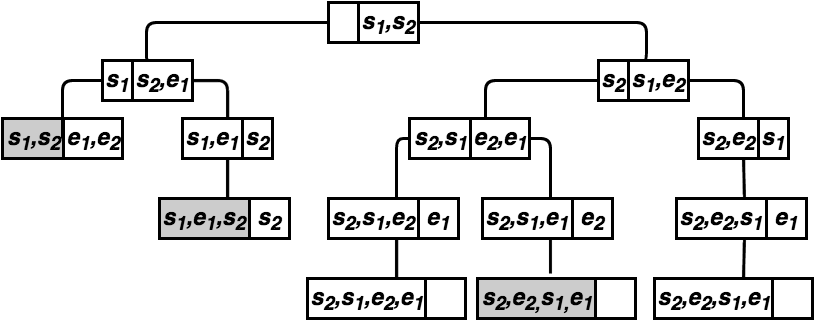
\includegraphics[width=0.75\columnwidth]{fig/bAndb.png}
	\vspace{-0mm}\caption{Illustration of \cref{algo:can_schedule}} \vspace{-2mm} \label{fig:bAndb}
\end{figure}\vspace{-0mm}

\vspace{-2mm}
\begin{algorithm}
	\caption{GetProfit($v, schedule, startTime$)}
	\label{algo:get_profit}
	\begin{algorithmic}[1]
		\REQUIRE \emph{schedule} is an ordered list of pick-up/drop-off points of driver $v$ and \emph{startTime} is the current time.
		\ENSURE the $profit$ of performing the input $schedule$ at time $startTime$. If $schedule$ is not valid it returns $-\infty$
		\STATE $time \leftarrow startTime$
		\STATE $loc \leftarrow v.$loc\label{ln:loc}
		\STATE $distance \leftarrow 0$
		\FOR{$p$ \textbf{in} $schedule$}
		\STATE $trip \leftarrow$ ShortestPath($loc, p$.loc)
		\STATE $distance \pluseq$ Distance($trip$)
		\STATE $time \pluseq$ TravelTime($trip$)
		\IF{$p$.type $==$ pick-up point}
		\IF{$time > p$.req.req\_time $ + $ p.req.w}\label{ln:mwt}
		\RETURN $-\infty$
		\ENDIF
		\STATE $pickUp[p$.req$]\leftarrow distance$
		\ENDIF
		\IF{$p$.type $ == $ drop-off point}
		\STATE $\Delta d \leftarrow distance - pickUp[p$.req$]$
		\IF{$\Delta d > p$.req.$\epsilon \times p$.req.sp}\label{ln:mad}
		\RETURN $-\infty$
		\ENDIF
		\STATE $fare \pluseq p$.req.f($\Delta d$) $\times$ F($p$.req.sp)\label{ln:delta}
		\STATE $cost \leftarrow v$.g($distance$)\label{ln:dprof}
		\ENDIF
		\STATE $loc \leftarrow p.loc$
		\ENDFOR
		\STATE $profit \leftarrow fare - cost$
=======
Once a driver is notified of a new request, it has to compute a bid. The bid each driver generates reflects the profit the system can gain if the request is assigned to that driver. Once the ride-sharing application receives the request, it generates a bid and submits the bid to the server. Once a new request is assigned to a diver, he will be notified with an updated schedule. This means that the human driver's interaction with APART is limited to configuring his profile on the ride-sharing application.

%\begin{algorithm}[!h]
%\caption{ComputeBid($v, r, time$)}
%\label{algo:comp_bid}
%\begin{algorithmic}[1]
%\REQUIRE $v$ is a driver, $r$ is a new request and $time$ is the current time.
%\ENSURE additional $profit$ that $v$ can generate by accepting $r$
%\STATE $src = \lbrace r'.s | r' \in v.schedule \rbrace$ 
%\STATE $src.$add$(r.s)$
%\STATE \small{$profit_n, schedule = $FindBestSchedule$(\emptyset, src, -\infty, \emptyset,  time)$} \label{ln:fbs}
%\STATE $profit_c, cost_c = $GetProfitAndCost$(v.schedule, time)$ \label{ln:gps}
%\RETURN $profit_n - profit_c$
%\end{algorithmic}
%\end{algorithm}
%
%\vspace{-.2in}
%
%\begin{algorithm}[!h]
%\caption{GetProfitAndCost($schedule, start$)}
%\label{algo:get_profit}
%\begin{algorithmic}[1]
%\REQUIRE \emph{schedule} is an ordered list of pick-up/drop-off points and \emph{start} is the current time.
%\ENSURE a pair of ($profit, cost$) of performing the input schedule. If the input schedule is not valid it returns ($-\infty, \infty$)
%\STATE $time = start$
%\STATE $loc = v.$loc\label{ln:loc}
%\STATE $trip = 0$
%\FOR{$p$ \textbf{in} $schedule$}
%	\STATE $path =$ ShortestPath($loc, p$.loc)
%	\STATE $trip \pluseq$ Distance($path$)
%	\STATE $time \pluseq$ TravelTime($path$)
%	\IF{$p$.type $= start$}
%		\IF{$time > p$.req.req\_time $+ p$.req.w}
%			\RETURN $-\infty$
%		\ENDIF
%		\STATE $pickUp[p$.req$]=trip$
%	\ENDIF
%	\IF{$p$.type $= end$}
%		\STATE $\delta d = trip - pickUp[p$.req$]$
%		\STATE $fare \pluseq p$.f($\delta d$) $\times$ F($p$.req.sp)
%		\STATE $cost = v$.g($trip$)\label{ln:dprof}
%	\ENDIF
%\ENDFOR
%\STATE $profit = fare - cost$
%\RETURN $profit, cost$
%\end{algorithmic}
%\end{algorithm}
%
%\cref{algo:comp_bid} outlines the bid computation process. The \textit{FindBestSchedule()} method takes a list of pick-up locations of requests and finds the best valid schedule for those requests (line~\ref{ln:fbs}). The reason \textit{FindBestSchedule()} is initially called with only the pick-up locations is to guarantee, for every request its pick-up locations is scheduled before its drop-off locations. In \cref{algo:can_schedule}, once the pick-up location of a request is scheduled, its drop-off location is added to list of remaining nodes to be scheduled. The variable $profit_n$ is the total profit of the best valid schedule that contains $r$. However the profit of $v$'s current schedule should be deducted from $profit_n$ to give the additional profit $v$ can generate by accepting $r$. The \textit{GetProfitAndCost()} method computes the profit and cost of \textit{v}'s current schedule (line~\ref{ln:gps}).
%
%%At each point in time, every driver has a schedule $s$. For every request $r_j \in s$, the driver can determine $r_j$'s incurred detour in $s$. Subsequently, using \cref{eq:fare,eq:payment,eq:profit} the driver can compute the profit it makes for APART.
%
%\cref{algo:get_profit} outlines the process of determining the profit each driver can generate if he starts executing the input \textit{schedule} at time \textit{start}. Each driver $v$ runs this algorithm locally and hence, $v.loc$ (line~\ref{ln:loc}) and $v.g()$ (line~\ref{ln:dprof}) refer to $v$'s current location and profile, respectively. Also, whether $p$ is a pick-up or drop-off point, in \cref{algo:get_profit} $p.req$ refers to the request for which $p$ is one of the end points. \cref{algo:get_profit} goes through the nodes in \textit{schedule} one by one and for every drop-off node, computes the traveled distance from when the pick-up node was passed and using \cref{eq:fare,eq:payment,eq:profit}, \cref{algo:get_profit} can compute the profit and cost of \textit{schedule}. If the input \textit{schedule} is not valid, the algorithm returns $-\infty$ and $\infty$ as the profit and cost, respectively.
%
%\begin{algorithm}[!ht]
%\caption{FindBestSchedule($f, r, bp, bs, start$)}
%\label{algo:can_schedule}
%\begin{algorithmic}[1]
%\REQUIRE \emph{f} and \emph{r} are lists of pick-up/drop-off points that have been added and to be added to a valid schedule, respectively. \emph{bp} and \emph{bs} are the best profit and corresponding schedule observed so far and \emph{start} is the current time.
%\ENSURE $bp, bs$ as the best profit and corresponding schedule for input points is a valid schedule exists. Otherwise $-\infty, \emptyset$
%\IF{$f$.size $+ r$.size $ > v$.n $\times 2$}
%	\RETURN $bp, bs$
%\ENDIF
%\FOR{$p$ \textbf{in} $r$}
%	\STATE $f' = f$
%	\STATE $f'$.add($p$)
%	\STATE $p, c =$ GetProfitAndCost($f', start$)
%	\IF{$p \neq -\infty$ and $p \geq bp$}
%		\STATE $r' = r$
%		\STATE $r'$.remove($p$)
%		\IF{$p$.type $= start$}
%			\STATE $r'$.add($p$.req.end)\label{ln:dropoff}
%		\ENDIF
%		\IF{$r'$.size $= 0$}
%			\RETURN $p, f'$
%		\ENDIF
%		\STATE $p, s =$ FindBestSchedule($f', r', bp, bs, start$)
%		\IF{$p > bp$}
%			\STATE $bs = s$
%			\STATE $bp = p$
%		\ENDIF
%	\ENDIF
%\ENDFOR
%\RETURN $bp, bs$
%\end{algorithmic}
%\end{algorithm}
%
%The first step in computing a bid is to find a potential valid schedule. If multiple such schedules exist, the one which generates maximum profit should be selected. In order to find a valid schedule, each driver runs a branch and bound algorithm outlined in \cref{algo:can_schedule}. The algorithm recursively performs an exhaustive search to find the best valid schedule. The variable $f$ is the set of nodes that have already been added to the schedule and $r$ is the set of remaining nodes. In each call, one node from $r$ is added to $f$. Every time a new node is added to $f$, the algorithm checks if $f$, which is a partial schedule, is valid or not. If not valid, it does not proceed further on that branch and backtracks to one level higher. The algorithm starts by only pick-up nodes of the requests in $r$ to ensure the pick-up node of a request is scheduled before its drop-off node. Once the pick-up node of a request is added to $f$, the drop-off node of the same request is added to $r$ (Line~\ref{ln:dropoff}).
%
%Once drivers submit their bids, the server selects the driver with the highest bid as the winner and assigns the new request to that. Assuming driver $v$ wins the auction, his reward for serving the request is the same amount as $cost_v$, based on which he determined the bid value. Also, upon assigning the new request to $v$, the service providers increases its revenue by $b_v$.


%%%%%%
%%% Ding's vesion of computing bid.
\begin{algorithm}[!h]
	\caption{ComputeBid($v, r, time$)}
	\label{algo:comp_bid}
	\begin{algorithmic}[1]
		\REQUIRE $v$ is a driver, $r$ is a new request and $time$ is the current time.
		\ENSURE additional $profit$ that $v$ can generate by accepting $r$
		\STATE $src = \lbrace r'.s | r' \in v.schedule \rbrace$ 
		\STATE $src.$add$(r.s)$
		\STATE \small{$profit_{new}, schedule = v$.FindBestSchedule$(\emptyset, src, -\infty, \emptyset,  time)$} \label{ln:fbs}
		\STATE $profit_{old}= $GetProfit$(v.schedule, time)$ \label{ln:gps}
		\RETURN $profit_{new} - profit_{old}$
	\end{algorithmic}
\end{algorithm}\vspace{-1mm}

\cref{algo:comp_bid} outlines the bid computation process. First, it inserts the pick-up locations (including the new request's pick-up point) in the list named $src$ (lines 1-2). Subsequently, the algorithm calls \textit{FindBestSchedule} which finds the best valid schedule and its corresponding profit using \cref{algo:can_schedule}. Because each driver's bid is the \textit{additional} profit that the new request can generate for the platform, we calculate $profit_{old}$ using \cref{algo:get_profit} for $v$'s original schedule (line~\ref{ln:gps}). Hence, the additional profit that $v$ can generate by accepting $r$ is the difference between $profit_{new}$ and $profit_{old}$. The reason \textit{FindBestSchedule} is initially called with only the pick-up locations is to guarantee, for every request its pick-up location is scheduled before its drop-off location. 

\begin{algorithm}[!ht]
	\caption{FindBestSchedule($f, r, bp, bs, start$)}
	\label{algo:can_schedule}
	\begin{algorithmic}[1]
		\REQUIRE \emph{f} and \emph{r} are lists of pick-up/drop-off points that have been added and to be added to a valid schedule, respectively. \emph{bp} and \emph{bs} are the best profit and corresponding schedule observed so far and \emph{start} is the current time.
		\ENSURE $bp, bs$ as the best profit and corresponding schedule for input points if a valid schedule exists. Otherwise $-\infty, \emptyset$
		\IF{$f$.size $+ r$.size $ > v$.n $\times 2$}
		\RETURN $bp, bs$
		\ENDIF
		\FOR{$p$ \textbf{in} $r$}
		\STATE $f' = f$
		\STATE $f'$.add($p$)
		\STATE $p =$ GetProfit($this, f', start$)
		\IF{$p \neq -\infty$}
		\STATE $r' = r$
		\STATE $r'$.remove($p$)
		\IF{$p$.type $= start$}
		\STATE $r'$.add($p$.req.end)\label{ln:dropoff}
		\ENDIF
		\IF{$r'$.size $= 0$}
		\RETURN $p, f'$
		\ENDIF
		\STATE $p, s =$ FindBestSchedule($f', r', bp, bs, start$)
		\IF{$p > bp$}
		\STATE $bs = s$
		\STATE $bp = p$
		\ENDIF
		\ENDIF
		\ENDFOR
		\RETURN $bp, bs$
	\end{algorithmic} \vspace{-1mm}
\end{algorithm}

We now explain how to find the most profitable schedule in \cref{algo:can_schedule}. The idea is to enumerate every valid schedule, calculate its profit and choose the most profitable one. Therefore, the algorithm recursively performs an exhaustive search to find the best valid schedule. Given the set of nodes that have already been added to the schedule(i.e., set $f$), and the remaining nodes(i.e., set $r$), at each iteration of \cref{algo:can_schedule} (lines 4-23), one node from $r$ is added to $f$ (lines 5-6). Each time a new node is added to $f$, the algorithm checks whether this partial schedule is valid. If the partial schedule is invalid, \textit{GetProfit} in line 7 returns $-\infty$ and the search continues to the next branch. Otherwise, the variable $p$ contains the profit of the partial schedule $f$. Once the pick-up node of a request is added to $f$, the drop-off node of the same request is added to $r$ (line 11-12). If the remaining nodes get empty, the search on the current branch stops and the current branch's profit $p$ is returned (lines 14-15); otherwise, it recursively checks the new branch $r'$ (line 17). The best profit is updated once the search finds a profit $p$ higher than the best profit seen so far $bp$ (lines 18-20). 

Figure~\ref{fig:bAndb} shows an example of using \cref{algo:can_schedule} to find a best schedule with two requests $r_1$ and $r_2$. Each rectangle represents a node in the search tree, where the left and right sections contain the scheduled points and the remaining points, respectively (sets $f$ and $r$ in \cref{algo:can_schedule}). Initially the set $r$ is started with the two pick-up locations. Each time a new pick-up point (e.g., $s_1$) is scheduled and moved from the right section to the left, the corresponding drop-off point (e.g., $e_1$) will be added to the right section. The shaded rectangles contain an invalid partial schedule in the left section and hence, the tree doesn't expand under them. The search continues until all the branches have been visited and the complete schedule with the highest profit is returned.

\begin{figure}[!ht]
	\centering
	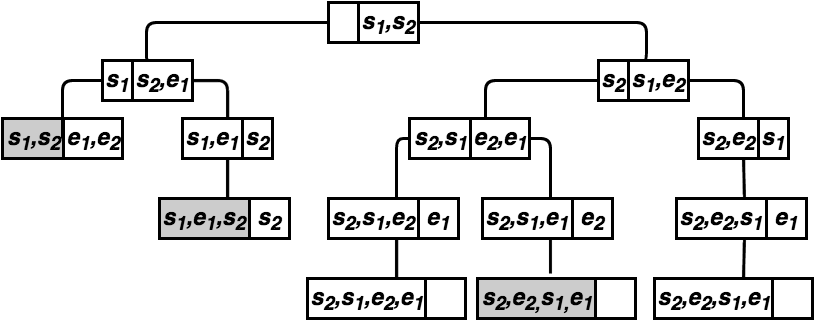
\includegraphics[width=0.75\columnwidth]{fig/bAndb.png}
	\vspace{-0mm}\caption{Illustration of \cref{algo:can_schedule}} \vspace{-2mm} \label{fig:bAndb}
\end{figure}\vspace{-0mm}

\begin{algorithm}
	\caption{GetProfit($v, schedule, start$)}
	\label{algo:get_profit}
	\begin{algorithmic}[1]
		\REQUIRE \emph{schedule} is an ordered list of pick-up/drop-off points of driver $v$ and \emph{start} is the current time.
		\ENSURE the $profit$ of performing the input $schedule$ at time $start$. If $schedule$ is not valid it returns $-\infty$
		\STATE $time = start$
		\STATE $loc = v.$loc\label{ln:loc}
		\STATE $distance = 0$
		\FOR{$p$ \textbf{in} $schedule$}
		\STATE $trip =$ ShortestPath($loc, p$.loc)
		\STATE $distance \pluseq$ Distance($trip$)
		\STATE $time \pluseq$ TravelTime($path$)
		\IF{$p$.type $= start$}
		\IF{$time > p$.req.req\_time $+ p$.req.w}\label{ln:mwt}
		\RETURN $-\infty$
		\ENDIF
		\STATE $pickUp[p$.req$]=distance$
		\ENDIF
		\IF{$p$.type $= end$}
		\STATE $\delta d = distance - pickUp[p$.req$]$
		\IF{$\delta d > p$.req.$\epsilon \times p$.req.sp}\label{ln:mad}
		\RETURN $-\infty$
		\ENDIF
		\STATE $fare \pluseq p$.f($\delta d$) $\times$ F($p$.req.sp)\label{ln:delta}
		\STATE $cost = v$.g($distance$)\label{ln:dprof}
		\ENDIF
		\ENDFOR
		\STATE $profit = fare - cost$
>>>>>>> 46f67d188a36b6f09f72c25697c415296ddf3444
		\RETURN $profit$
	\end{algorithmic} 
\end{algorithm}

<<<<<<< HEAD
\cref{algo:get_profit} computes the profit driver $v$ can generate by completing $schedule$ at $startTime$. Each driver $v$ runs this algorithm locally, and hence, $v.loc$ (line~\ref{ln:loc}) and $v.g$ (line~\ref{ln:dprof}) refer to $v$'s current location and profile, respectively. Also, for any node $p$ in the schedule, $p$.req and $p$.req.sp refer to the corresponding request of node $p$ and the shortest path for that request, respectively. \cref{algo:get_profit} iterates through the nodes in \textit{schedule} one by one keeping track of the added $time$ and $distance$. Each node is either a pick-up node or a drop-off node. For pick-up nodes, the algorithm checks if the maximum wait time constraint is violated (line~\ref{ln:mwt}). For every drop-off node, the detour constraint is checked (line~\ref{ln:mad}). If the check is successful, the algorithm computes the actual travel distance for the request and determines the incurred detour (line~\ref{ln:delta}). After computing the detour, the algorithm computes the added fare and cost using \cref{eq:fare,eq:payment,eq:profit}. If the input \textit{schedule} is not valid, the algorithm returns $-\infty$ as the profit.

Once drivers submit their bids, the server selects the driver with the highest bid and assigns the new request to that driver.
=======
\cref{algo:get_profit} computes the profit driver $v$ can generate by completing $schedule$ at time $start$. Each driver $v$ runs this algorithm locally, and hence, $v.loc$ (line~\ref{ln:loc}) and $v.g()$ (line~\ref{ln:dprof}) refer to $v$'s current location and profile, respectively. Also, for any node $p$ in the schedule, $p$.req and $p$.req.sp refer to the corresponding request of node $p$ and the shortest path for that request, respectively. \cref{algo:get_profit} iterates through the nodes in \textit{schedule} one by one keeping track of the added $time$ and $distance$. Each node is either a pick-up node or a drop-off node. For pick-up nodes, the algorithm checks if the maximum wait time constraint is violated (line~\ref{ln:mwt}). For every drop-off node, the detour constraint is checked (line~\ref{ln:mad}). If the check is successful, the algorithm computes the actual travel distance for the request and determines the incurred detour (line~\ref{ln:delta}). After computing the detour, the algorithm computes the added fare and cost using \cref{eq:fare,eq:payment,eq:profit}. If the input \textit{schedule} is not valid, the algorithm returns $-\infty$ as the profit.

Once drivers submit their bids, the server selects the driver with the highest bid as the winner and assigns the new request to that driver.
>>>>>>> 46f67d188a36b6f09f72c25697c415296ddf3444
%The drives cost (income) is determined similar to \cref{algo:get_profit}.

%\subsection{Payments in \fname}

%Once every driver submits his bid, the server selects the driver with the highest bid as the winner and allocates the new request to him. Assuming driver $v$ wins the auction with probability $p_v$, his expected compensation is: 

%\begin{equation*}
%E[comp_v] = p_v.Comp_v(win) + (1 - p_v).Comp_v(loose)
%\end{equation*}

%Where $Comp_v()$ gives the compensation driver $v$ receives for winning or loosing the auction. Intuitively, in the case of winning, $v$ gets compensated the same amount as $cost_v$ based on which he determined his bid and receives $\$0$ for loosing, i.e., $E[comp_v] = p_v.cost_v$. We call this payment model first-price, since the compensation the winner receives is only based on the highest bid.

%Earlier we mentioned that the human driver has no interaction with \fname with regard to computing and submitting a bid. However, depending on how the human driver customizes his profile $g()$, he can affect his $cost$ computation and consequently, the bid value~\footnote{Hereafter, when we say the driver increases/decreases his bid, we mean he does it indirectly by customizing his profile}. For example, assume $v_i$ is the winner of the auction with bid $b_i$ and the second highest bid is $b_j$. In theory, if $v_i$ changes his profile such that his bid becomes $b_i - \epsilon (\epsilon < b_i - b_j)$, he will still be the winner of the auction and has gets compensated $\$\epsilon$ more than when his bid was $b_i$. In practice, however, $v_i$ does not know the \textit{actual} value of any other driver's bid. Therefore, for every driver there is a trade-off between lowering the value of the bid and the probability of being the winner. To maximize his compensation, a rational driver makes his bid as close as possible to the \textit{expected} value of the second highest bid. The details of how each driver can compute this expected value is out of the scope of this paper and more details can be found in \cite{Vickery61}.

%In order to facilitate the bid computation process for workers, \fname adopts a payment model in which the drivers do not benefit from increasing/decreasing their cost and bid values. The compensation of the winner driver in \fname is computed as:

%\begin{equation*}
%comp_i = cost_i + (bid_i - bid_j)
%\end{equation*}

%\noindent Where $v_i$ is the driver with the highest bid and $v_j$ is the driver with the second highest bid. Since the compensation depends on not only the highest bid but also the second highest bid, we call it the second-price model. Following we first prove that with the second-price model, each driver can maximize his compensation by configuring their profiles such that it results in the \textit{minimum} cost that is economical for him to participate in the system. Next we show that in the second-price payment model, not only we get the same rider to driver assignments, but also the final revenue of \fname in both model remains the same.

%\begin{theorem}
%In the second-price payment model, a driver has no incentive to configure his profiles such that his resulting cost is either lower or higher than his minimum cost.
%\end{theorem}

%\begin{theorem}
%Both the first-price and second-price payment model result in the same rider to driver assignment and generate the same revenue.
%\end{theorem}